\documentclass{paper}

%\usepackage{times}
\usepackage{epsfig}
\usepackage{graphicx}
\usepackage{amsmath}
\usepackage{amssymb}
\usepackage{color}
\usepackage{caption}
\usepackage{subcaption}


% load package with ``framed'' and ``numbered'' option.
%\usepackage[framed,numbered,autolinebreaks,useliterate]{mcode}

% something NOT relevant to the usage of the package.
\setlength{\parindent}{0pt}
\setlength{\parskip}{18pt}
\graphicspath{{images/}}


\usepackage[latin1]{inputenc}
\usepackage[T1]{fontenc}


\usepackage{listings}
\lstset{%
   language=R,
   basicstyle=\small\ttfamily,
   frame=single
}



\title{Assignment 6}



\author{Jenni Simon\\09-116-005}
% //////////////////////////////////////////////////


\begin{document}



\maketitle


% Add figures:
%\begin{figure}[t]
%%\begin{center}
%\quad\quad   \includegraphics[width=1\linewidth]{ass2}
%%\end{center}
%
%\label{fig:performance}
%\end{figure}


\paragraph{Exercise 1}

Please refer to the provided code for the implementation of the function...

\paragraph{Exercise 2}

The values chosen for $k$ were $k_{Computer}=1$ and $k_{Cars}=26$. The choice was based on a comparison of the resulting Sum of Residuals Squared (SRS) obtained on a held out test-set. Figures \ref{fig:comp} and \ref{fig:cars} show the squared residuals obtained on both test-sets.

\begin{figure}[h]
\begin{center}
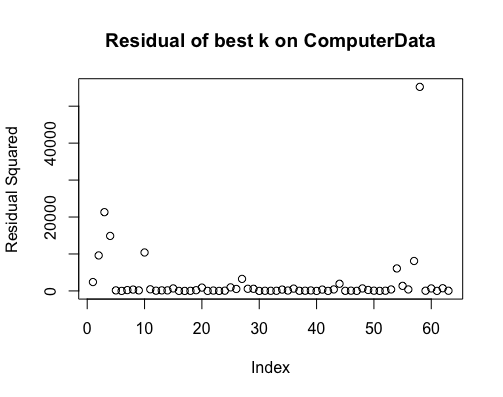
\includegraphics[width=0.8\linewidth]{comp}
\end{center}
\caption{Residuals squared on the Computer data test-set. }
\label{fig:comp}
\end{figure}

\begin{figure}[h]
\begin{center}
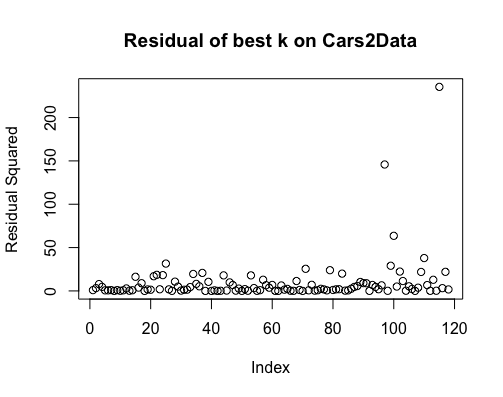
\includegraphics[width=0.8\linewidth]{cars}
\end{center}
\caption{Residuals squared on the Cars data test-set. }
\label{fig:cars}
\end{figure}



\end{document}
